\subsection{LMFormer}
\label{ssec:lmformer}

LMFormer~\cite{lmformerYadav2025} is a fully query-centric, transformer-based architecture for joint multi-agent trajectory forecasting. It ingests both static lane segments and dynamic agent motion vectors in their local frames, embeds them via learnable Fourier features, and processes them through specialized self- and cross-attention blocks before recurrently decoding multiple future modes. The high-level architecture is shown in \autoref{fig:lmformer_arch}.

\begin{figure}[ht]
  \centering
  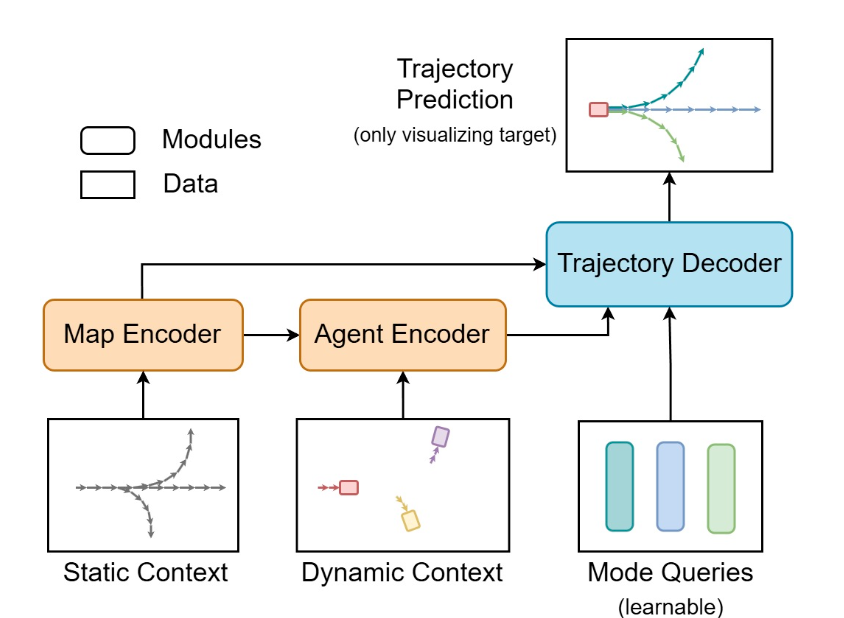
\includegraphics[width=0.8\textwidth]{figures/lmformer_arch.png}
  \caption{LMFormer overall architecture: query-centric encoding of static and dynamic contexts, followed by a transformer encoder and a recurrent cross-attention decoder.}
  \label{fig:lmformer_arch}
\end{figure}

\paragraph{Learnable Fourier Embeddings.}
All input features—lane segment lengths and motion-vector lengths/orientations—are first lifted into a high-dimensional space via learnable Fourier embeddings~\cite{li2021llearnableFourier}. By applying sinusoidal transforms to invariant scalars, these embeddings enrich expressivity without breaking \(\mathrm{SE}(2)\!\rtimes\!\mathbb{R}\) invariance.

\paragraph{Transformer Encoder.}
The encoder alternates \emph{static} and \emph{dynamic} branches, each customized to its context:

\begin{itemize}[leftmargin=*]
  \item \textbf{Map (Lane) Encoder:}
        Applies multi-headed self-attention over \(N_L\) lane-segment tokens, each equipped with its Fourier embedding. This block captures long-range lane interactions and yields \emph{lane encodings} of shape \((N_L, D)\).
  \item \textbf{Agent Encoder:}
        Stacks three attention modules over \(N_a\) agent tokens with \(T_{\text{in}}\) timesteps:
        \begin{enumerate}
          \item Temporal self-attention across time steps for each agent.
          \item Agent-agent cross-attention to model social interactions.
          \item Agent-lane cross-attention to fuse static context.
        \end{enumerate}
        The encoder repeats this triad \(N\) times, producing \emph{agent encodings} of shape \((N_a, T_{\text{in}}, D)\).
\end{itemize}

\begin{figure}[ht]
  \centering
  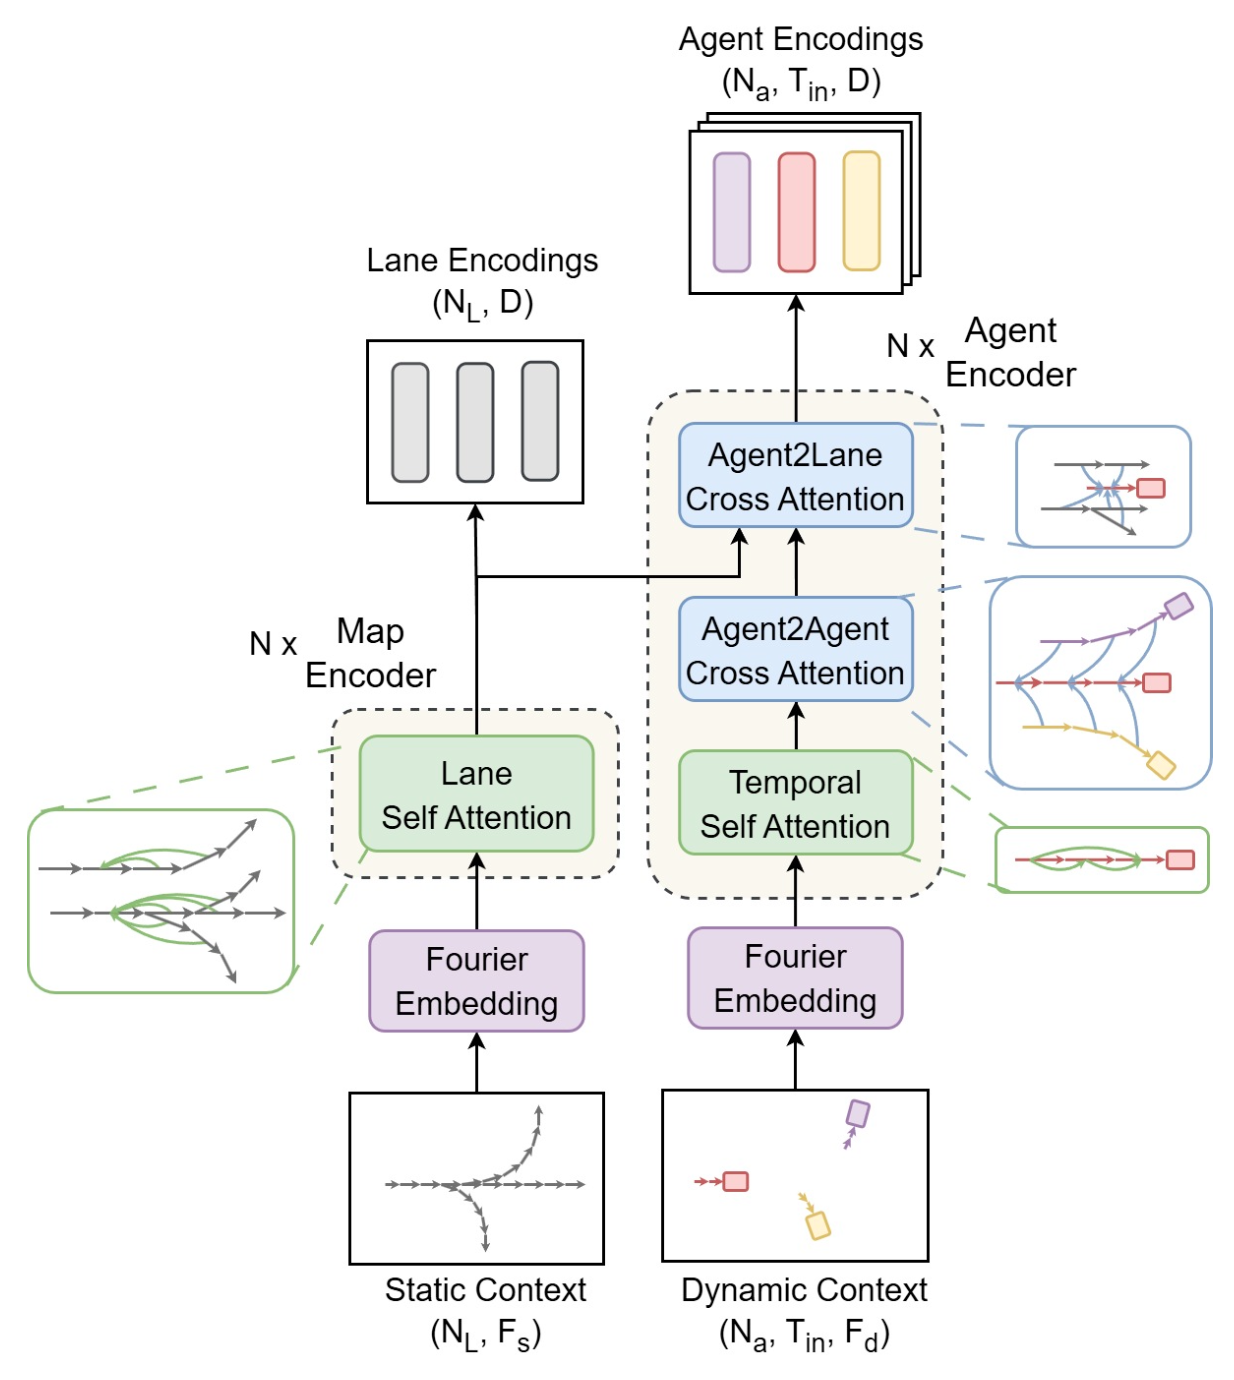
\includegraphics[width=0.85\textwidth]{figures/lmformer_arch_encorder.png}
  \caption{LMFormer encoder: (left) learnable Fourier embeddings, (center) lane self-attention, (right) agent temporal and cross-attentions.}
  \label{fig:lmformer_arch_encoder}
\end{figure}

\paragraph{Recurrent Cross-Attention Decoder.}
LMFormer employs a recurrent decoding loop for \(T_{\text{out}}\) future steps, using three \emph{mode queries} per agent (see \autoref{ssec:caspformer}). At each step, the decoder executes:

\begin{enumerate}[leftmargin=*]
  \item \textbf{Mode2Temporal Cross-Attention:} Each mode query attends to the agent encodings to propagate temporal context.
  \item \textbf{Mode2Agent Cross-Attention:} Queries attend across agents to capture social dependencies in the predicted futures.
  \item \textbf{Mode2Lane Cross-Attention:} Queries incorporate static lane information by attending to lane encodings.
\end{enumerate}

After each cross-attention block, the updated queries pass through an MLP head to predict incremental motion vectors. This loop is repeated \(T_{\text{out}}\) times, yielding mode-specific trajectories of shape \((M, N_a, T_{\text{out}}, 2)\). The decoder structure is illustrated in \autoref{fig:lmformer_arch_decoder}.

\begin{figure}[ht]
  \centering
  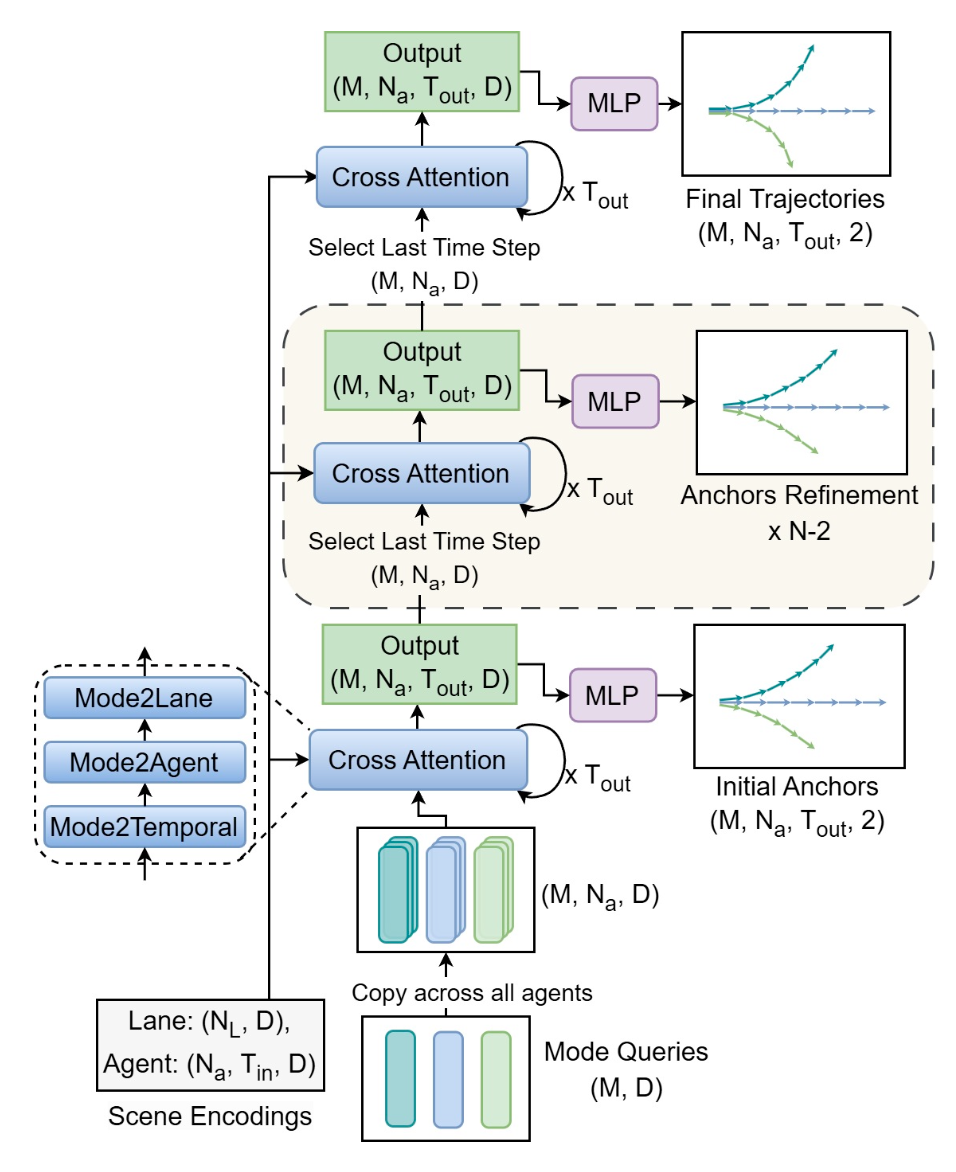
\includegraphics[width=0.85\textwidth]{figures/lmformer_arch_decoder.png}
  \caption{LMFormer decoder: recurrent mode-query cross-attention modules that iteratively generate future motion vectors.}
  \label{fig:lmformer_arch_decoder}
\end{figure}


\paragraph{Output representation.}
Following \cite{lmformerYadav2025}, every mode query ultimately predicts a
\emph{motion-vector chain}
\(
\mathcal{T}_{out}^{a,m}
  = \bigl[(V_1^{a,m},S_1^{a,m}),\dots,(V_{T'}^{a,m},S_{T'}^{a,m})\bigr],
\)
where \(V_t^{a,m}=[P_{t-1}^{a,m},P_t^{a,m}]\) is a displacement vector and
\(S_t^{a,m}\in\mathbb{R}^{2}\) its per-coordinate variance.
Each \(\langle V_t,S_t\rangle\) pair parameterises one component of a
\textbf{Laplacian mixture} density, which empirical work
has shown to match the heavy-tailed statistics of real human motion better than
Gaussian mixtures~\cite{zhou2022hivt,caspformerYadav2024}.  Because the
vectors are defined in their own query-centric frames and all network blocks
respect the symmetries summarised in \autoref{sssec:qc_geometric_perspective},
the \emph{complete} prediction set remains

\begin{itemize}[nosep,leftmargin=1.5em]
\item \textbf{permutation-equivariant} - shuffling agent indices merely reorders rows,
\item \textbf{\(SE(2)\)-invariant} - rotating/translating the world leaves the trajectories identical up to the same rigid transform, and
\item \textbf{time-shift invariant} - sliding the observation window by \(\tau\) steps does not change the latent scene tensor for the overlapping frames.
\end{itemize}

These properties allow the same cached scene encoding to serve \emph{all}
agents and \emph{all} successive frames, a capability absent in the
agent-centric CASP family.

\paragraph{Loss formulation.}
LMFormer re-uses the winner-takes-all loss from
\autoref{par:casp_loss_formulation} but supervises \emph{every} refinement
layer (except the first) to encourage coarse-to-fine anchors:
\begin{equation}
  \mathcal{L}
  = \lambda\,\mathcal{L}_{cls}
    + \sum_{n=2}^{N}\mathcal{L}_{reg}^{(n)},
  \label{eq:lm_loss}
\end{equation}
where \(N\) stacked decoder layers iteratively refine trajectories, and
\(\lambda\) balances classification against regression
\cite{lmformerYadav2025}.

\paragraph{Conceptual contributions and latent representations.}
\begin{enumerate}[leftmargin=*]
  \item \textbf{Lane-first static encoding.}  Restricting static context to
        lane segments lets the lane self-attention block build a compact,
        directed graph of drivability priors, avoiding CASPFormer's large BEV
        raster while keeping high geometric fidelity.
  \item \textbf{Recurrent anchor refinement.}  Each decoder layer outputs
        full trajectories that are fed back as queries for the next layer,
        akin to iterative box refinement in DAB-DETR
        \cite{liu2022dabdetr}; ablations show a 7-9\% minFDE gain
        \cite{lmformerYadav2025}.
  \item \textbf{Scene-consistent multi-agent decoding.}  Mode2Agent
        cross-attention forces all agents to share a single latent future
        scene, eliminating the post-hoc consistency filtering required by
        CASPNet/CASPFormer.
\end{enumerate}

\paragraph{Relation to CASPNet \& CASPFormer.}
CASPNet operates on raster grids and predicts per-pixel occupancies; CASPFormer adds deformable attention and vector outputs but retains an \emph{agent-centric} frame.  LMFormer discards the raster backbone entirely, embraces the query-centric paradigm, and gains strict symmetry compliance and parallel multi-agent decoding—at the cost of a larger key-value cache and higher VRAM demand (\( \approx \)2x CASPFormer on nuScenes).

\paragraph{Open questions.}
Future work could explore (i) sparse or deformable query-centric attention to reduce memory further, (ii) explicit physical feasibility constraints (e.g., maximum curvature, speed limits) inside the decoder, and (iii) domain adaptation layers to mitigate the intersection-centric bias observed when transferring from nuScenes to broader urban datasets\cite{lmformerYadav2025}.


\paragraph{Pros.}
\begin{itemize}[leftmargin=*, label=\greenoplus]
  \item Fully query-centric, preserving \(\mathrm{SE}(2)\!\rtimes\!\mathbb{R}\) invariance end-to-end.
  \item Joint multi-agent decoding with shared static context.
  \item Recurrent refinement yields temporally coherent, multi-modal trajectories.
\end{itemize}

\paragraph{Cons.}
\begin{itemize}[leftmargin=*, label=\redominus]
  \item Increased memory footprint due to storing per-agent, per-timestep keys/values.
  \item Decoder latency scales linearly with \(T_{\text{out}}\) and number of modes.
  \item Requires careful tuning of Fourier embedding frequencies to balance expressivity and stability.
\end{itemize}